\documentclass[18pt,a4paper]{article}

%preamble
\usepackage{hyperref}
\usepackage{graphicx}
\usepackage[utf8]{inputenc}
\usepackage{amsmath}
\usepackage{enumitem}
\usepackage{multirow}


\author{Md Shamsuzzoha Bayzid
, Mahjabin Nahar,
 Md Shariful Islam Bhuyan,\\
 and Md Saidur Rahman}
\title{CSE 300: Online Assignment}
\date{April 2021}

\usepackage{siunitx} % Required for alignment
\sisetup{
  round-mode          = places, % Rounds numbers
  round-precision     = 2, % to 2 places
}

\begin{document}

\maketitle
%\pagenumbering{arabic}

\section{Introduction}
This assignment has been designed to assess the preparation
 of the students in writing
 scientific articles using \LaTeX. 
  This assignment covers a variety of 
  components that arecommonly used in scientific 
  manuscripts.

\subsection{Figures}
We intend to put Figure \ref{fig:1} at the top of a page

\begin{figure}[t]
	\centering
	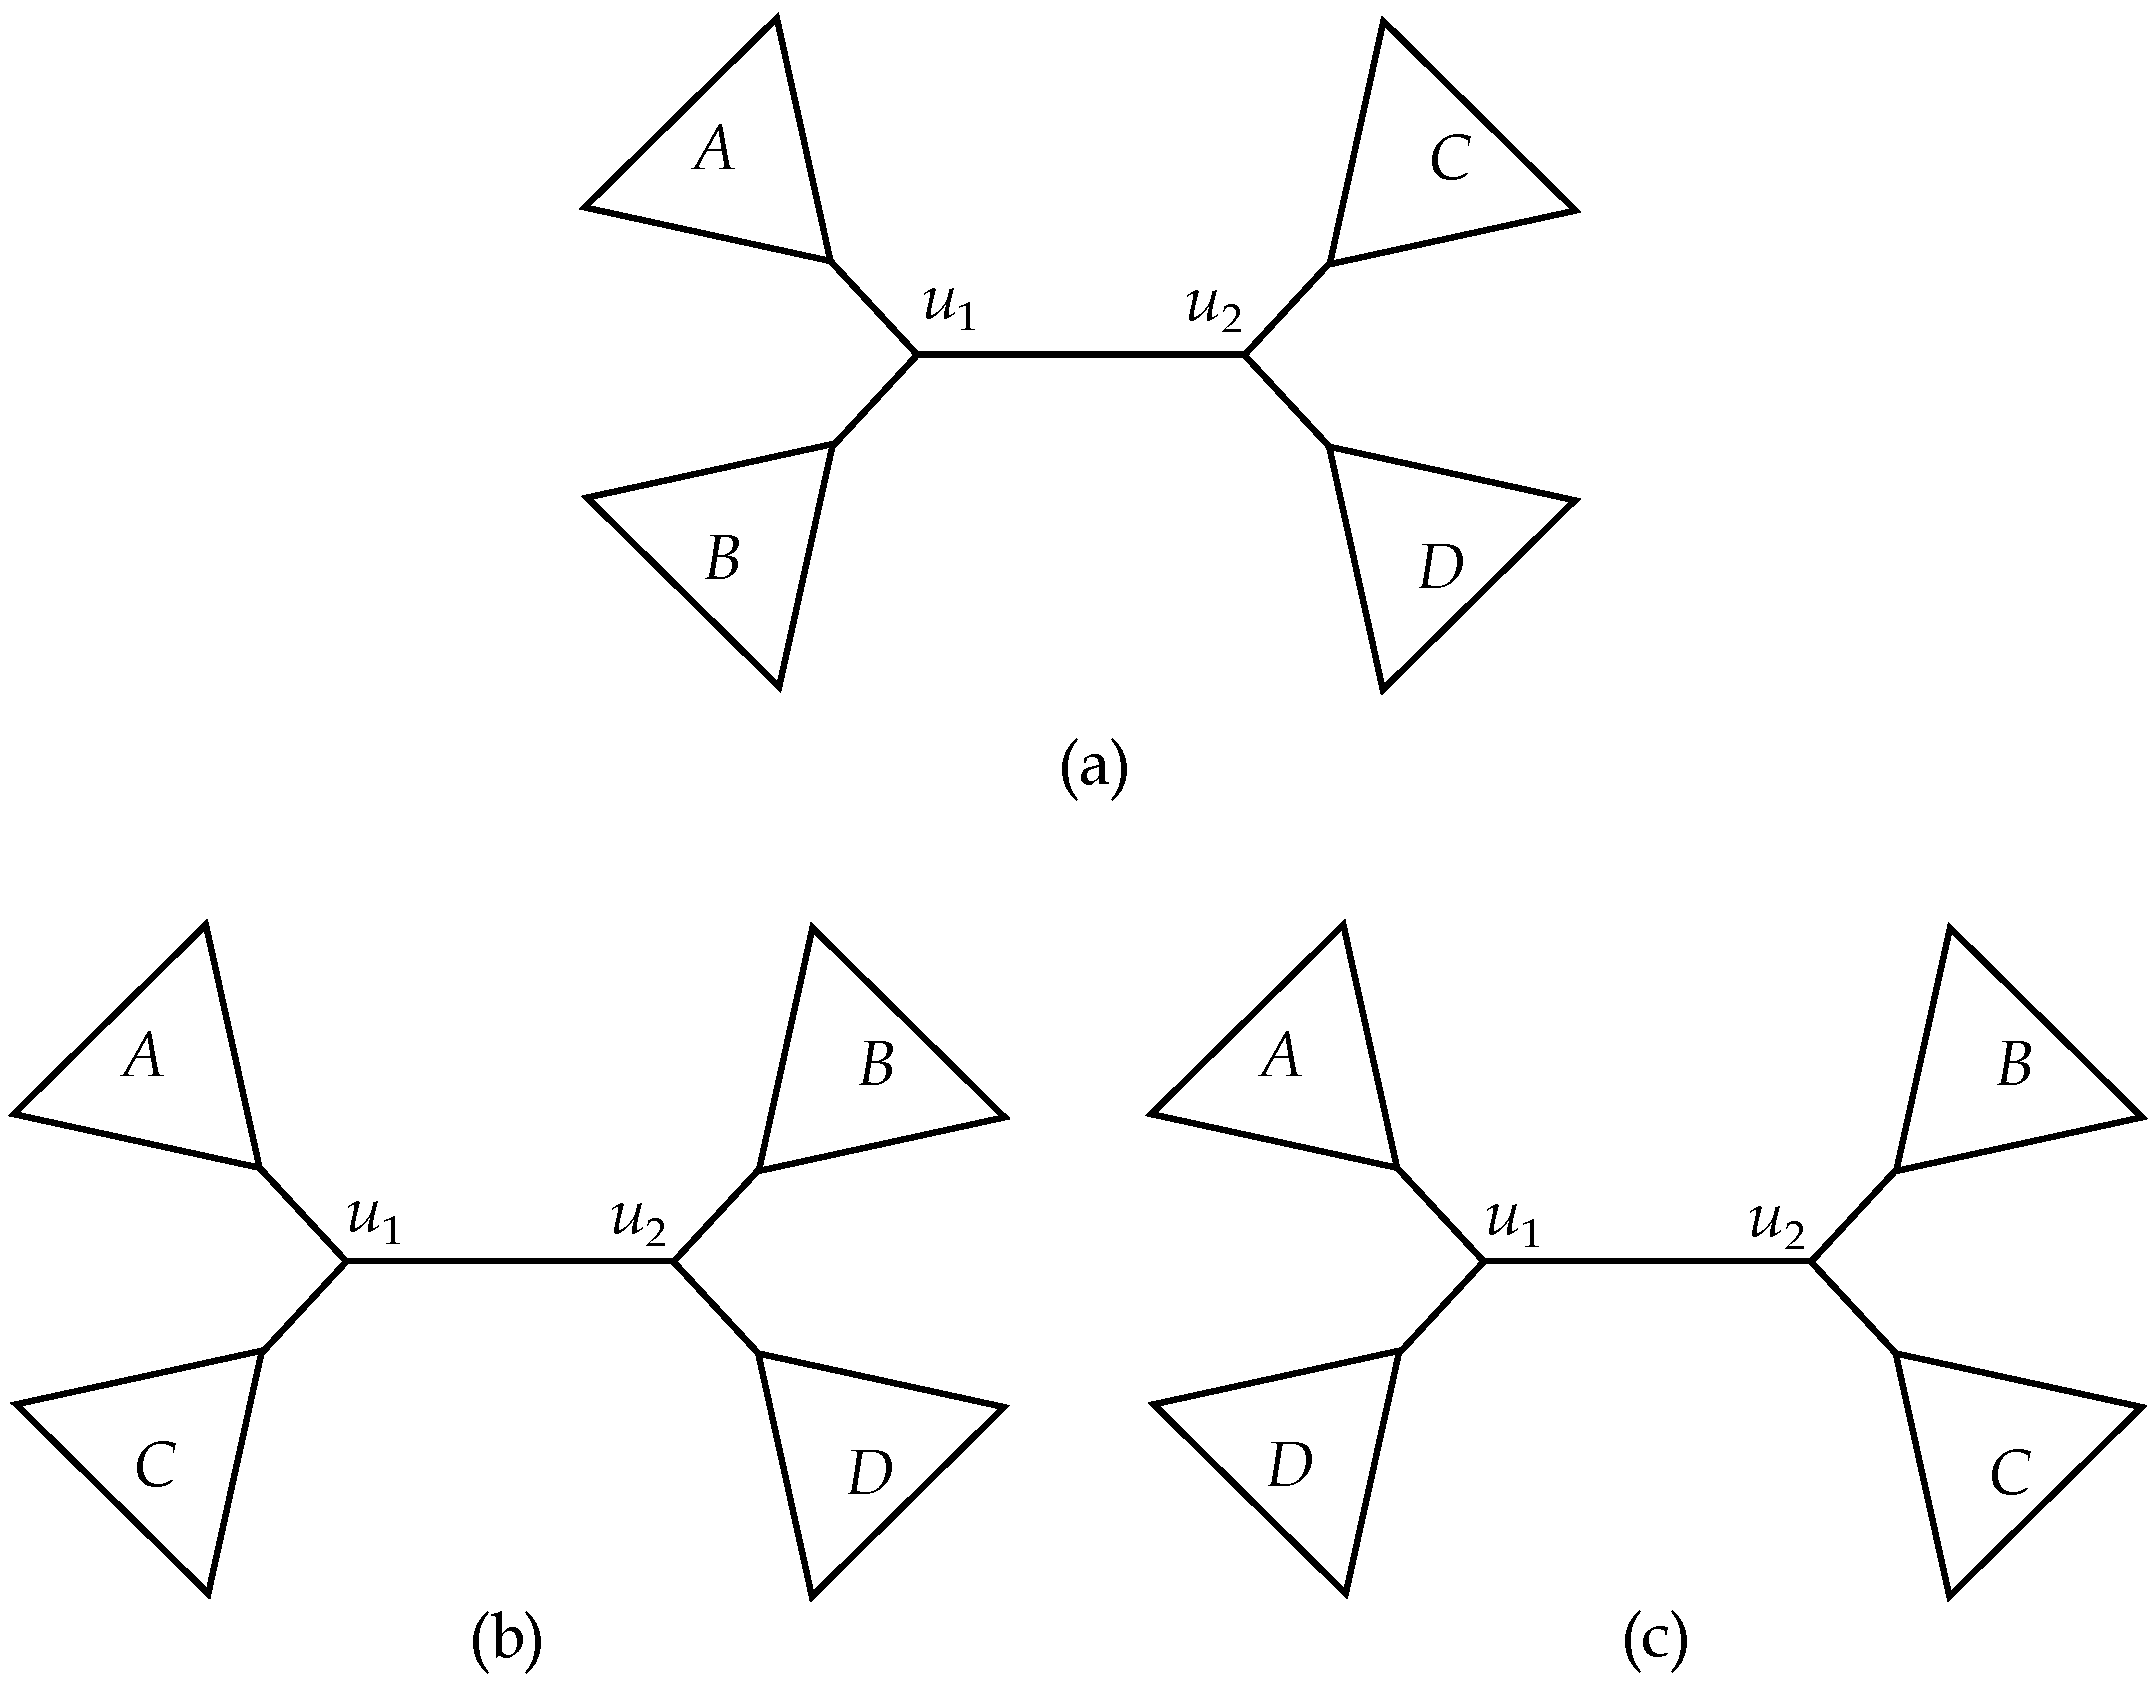
\includegraphics[scale = 0.3 , width = \linewidth ] {Figure3.pdf}
	\caption{ \textbf{Nearest Neighbor Interchange (NNI) move on an internal edge}.(a)A species tree $ST$, 
	and (b)-(c) the neighbors of $ST$ resulting from one NNI move on edge $e = (u_1, u_2)$.
	$A, B, C, \and D$ are the sets of taxa in the four subtrees 
	around edge $e$.}
	\label{fig:1}
\end{figure}

\subsection{Tables}
We wish to place Table 1 right here.

\begin{table}[h!]
	\label{one}
	\caption{\textbf{Optimization scores for Method-1 
	and Method-2 on different datasets covering 
	 various  model  conditions.}
	  We  show  average  scores  of  two  optimization 
	  criteria for various model conditions.\\}
	\begin{tabular}[h]{|l r| r r| r c|}
		\hline
		
		Dataset & 
		Model &
\multicolumn{2}{c}{Optimization Score 1} &
\multicolumn{2}{c}{Optimization Score 2} \\
		\cline{3-6}
			&
		condition &
		 Method-1 &
		Method-2 &
		Method-1 &
		Method-2 \\
		\hline
		\hline
		\multirow{4}{*}{D1}
		&
		$M_1$ &
		7,425.55 &
		770.00 &
		929.55 &
		10 \\
		&
		$M_2$ &
		7,657.00 &
		9,179.00 &
		716.15 &
		20 \\

		&
		$M_3$ &
		54.00 &
		9,007.15 &
		3,759.00 &
		30 \\

		&
		$M_3$ &
		74.00 &
		5567.15 &
		99.00 &
		25 \\
		\hline

		\multirow{3}{*}{D2} &
		$M_1$ &
		34.00 &
		273.15 &
		321.60 &
		34 \\

		&
		$M_2$ &
		357.00 &
		79.15 &
		321.60 &
		34 \\

		&
		$M_3$ &
		357.00 &
		79.15 &
		321.60 &
		34 \\
		\hline

	\end{tabular}
\end{table}

\subsection{Equations}
Let $n_1|n_2|n_3$ 
be  a  tripartition  defined  on  an  internal  node
$u$ of  a  binary  tree $T$. 
The number of tripartitions mapped to $u$ is given by Eqn. \ref{eqn}.

\begin{equation}
	\label{eqn}
	NQ(n_1,n_2,n_3) = \binom{n_1}{2} \binom{n_2}{1}
	\binom{n_3}{1} + \binom{n_2}{2} 
	\binom{n_1}{1} \binom{n_3}{1} + \binom{n_3}{2}
	\binom{n_1}{1} \binom{n_2}{1} 
\end{equation}

\section{Conclusions}
The major objectives of this assignment are listed below 
(please do not ignore the fontsizes).

\begin{description}
\item[1.] {\huge To assess the ability of 
the students in preparing manuscriptsin \LaTeX .
\item[2.] }{\large To see if the students have 
adequately practiced different aspects ofwriting in \LaTeX.
\item[3.] }{ \small To see if the students can add various basic components 
(e.g., tables, figures, equa-tions) to a \LaTeX manuscrip.
\item[4.] }{\tiny To see if the students can leverage the available materials
 (both offline and online) to dosomething which has not explicitly been taught
  in the class.}
\end{description}

\end{document}